\section{Central Processing Unit}

Il compito della CPU è quello di \textbf{eseguire i programmi} immagazzinati nella memoria centrale, leggendo le loro istruzioni ed eseguendole in sequenza.

La CPU opera in modo ciclico, ripetendo fino alla fine del programma le operazioni di \textbf{fetch-decode-execute}: acquisisce l'istruzione, la decodifica e la esegue

\begin{figure}[H]
    \centering
    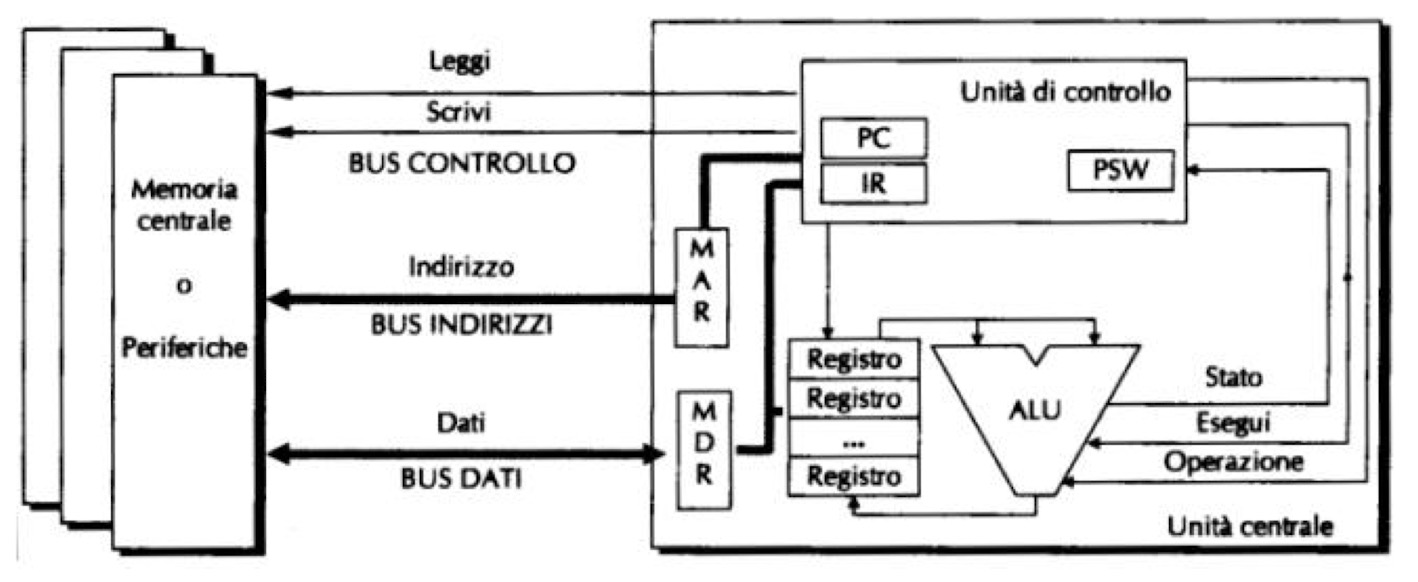
\includegraphics[width=0.55\linewidth]{assets/cpu-architecture.jpg}
\end{figure}

Una CPU è composta da:
\begin{sitemize}
    \item \textbf{Unità di controllo:} ha il compito di leggere le istruzioni e determinarne il tipo.
    \item \textbf{Arithmentic and Logic Unit (ALU):} Esegue le operazoni matematiche necessarie per l'esecuzione dell'istruzione.

    I dati devono partire dai registri e il risultato deve tornare nei registri, questo percorso viene detto \textit{data path}, ogni istruzione comporta l'esecuzione di uno o più cicli di \textit{data path}.
    \item \textbf{Registri:} Una memoria di piccole dimensioni che risiede all'interno del processore, viene utilizzata per memorizzare i risultati temporanei e le informazioni di controllo della CPU.

    \begin{note}
        Due registri particolarmente importanti sono l'Instruction Register (IR) che immagazzina l'istruzione corrente e il Program Counter (PC) che punta alla prossima istruzione.
    \end{note}

    \item \textbf{MDR:} è un registro a cui la ALU ha accesso diretto e che contiene momentaneamente i dati da/per la CPU.
    \item \textbf{MAR:} è un registro della CPU contenente l'indirizzo della locazione di memoria RAM in cui si andrà a leggere o scrivere un dato.
    \item \textbf{Bus di Controllo:} un bus che permette alla CPU di specificare che operazione deve svolgere sulla memoria.
    \item \textbf{PSW:} \textit{Program Status Word} i bit che forniscono informazioni sul risultato dell'ultima operazione eseguita. (overflow, carry, segno)
\end{sitemize}

Ogni ciclo di esecuzione si compone di alcuni passaggi:
\begin{sitemize}
    \item Il valore di PC viene copiato nel MAR
    \item La memoria scrive sul MDR il valore all'indice specificato dal MAR
    \item Il valore di MDR viene copiato sull'IR
    \item L'istruzione viene eseguita dall'ALU
    \begin{sitemize}
        \item Se l'istruzione richiede degli operandi essi devono essere inseriti nei registri attraverso MAR e MDR, similmente a quanto fatto per l'istruzione
    \end{sitemize}
    \item Terminata l'esecuzione il risultato viene scritto sul MDR e l'indirizzo di destinazione sul MAR, la memoria poi si occupa di copiare il valore.
    \item Si ricomincia dal primo punto con l'istruzione successiva.
\end{sitemize}
